\documentclass[a4paper,ft=14pt]{article}

\usepackage{color}
\usepackage{graphicx}
\usepackage{hyperref}
\usepackage[utf8]{inputenc}

\begin{document}
\begin{titlepage}
\title{ASP.NET Project}
\author{Mina Sameh Wadie Zaki \\ \texttt{2018 030 160} \\ Supervised by Eng Hadeer}
\date{\today}
\maketitle
\end{titlepage}

\section{Main Idea}
\begin{abstract}
This Project is about delivering free books, such as \href{pdfdrive.com}{pdfdrive} where you can find free educational or spiritual
books and maybe learn something.\\
The idea is a bit small, but I wanted to learn new things and improve and I felt like this idea is the 
best way to do so.
\end{abstract}

\section{Technology Used}
\begin{itemize}
	\item BootStrapMade
	\item Cypress
	\item Visual Studio 2010
	\item DataTables
\end{itemize}

I will first talk on the technologies I used and why I used them. \\
Of course this Project uses Asp.Net as its a main requirement, however I wanted to create a
I used for the website templates \href{https://bootstrapmade.com}{BootStrapMade} which used Bootstrap and JQuery 
to create beautiful Responsive Pages. \\
I used \href{https://www.cypress.io/}{cypress} to test out the pages End to End, meaning it will open the page and simulate user behavior, 
which was a big help in the project and I believe it was instrumental in helping me finish the project on time.\\
I used JQuery and \href{https://www.datatables.net/}{DataTables} to create beautiful DataTables, and ease the load off the backend as ASP isnt the "latest" anything anymore.



\section{Diagrams}

\subsection{ERD}
\noindent\makebox[\textwidth]{
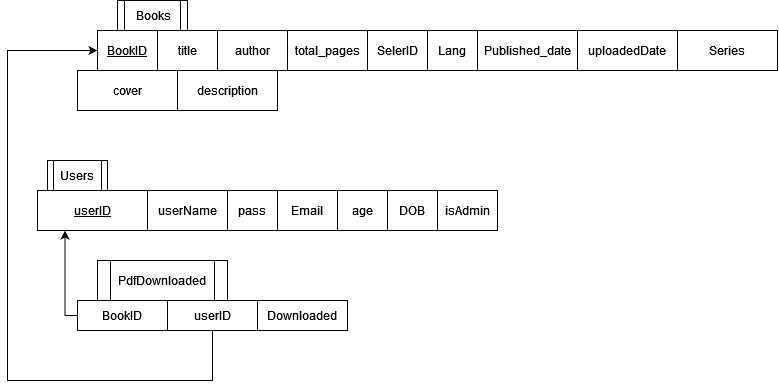
\includegraphics[width=\paperwidth]{C:/Users/Mina Sameh/Downloads/Tex/ERD.png}
}
\subsection{Context}
\noindent\makebox[\textwidth]{
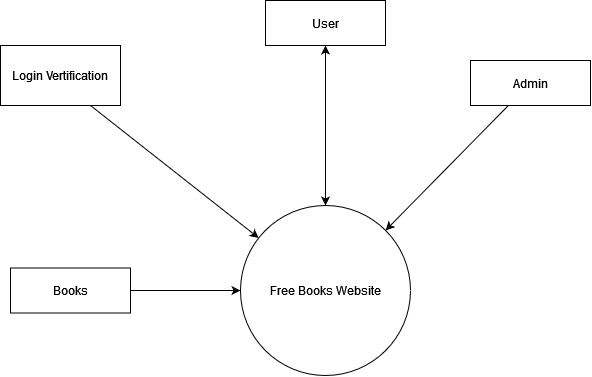
\includegraphics[width=\paperwidth]{C:/Users/Mina Sameh/Downloads/Tex/Context Diagram.png}
}

\subsection{Collabroation}
\noindent\makebox[\textwidth]{
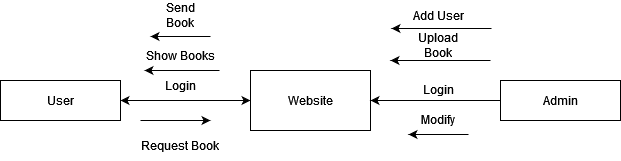
\includegraphics[width=\paperwidth]{C:/Users/Mina Sameh/Downloads/Tex/Collabration.png}
}
\subsection{DFD}
\noindent\makebox[\textwidth]{
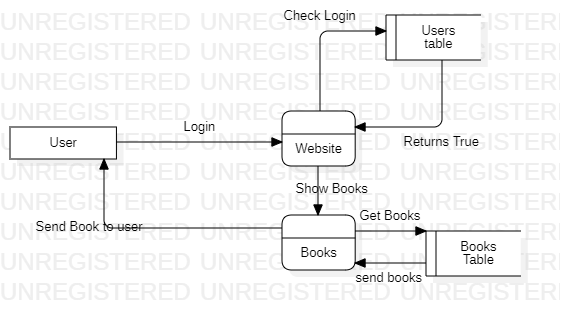
\includegraphics[width=\paperwidth]{C:/Users/Mina Sameh/Downloads/Tex/DFDDiagram1.png}
}
\subsection{Pert}
\noindent\makebox[\textwidth]{
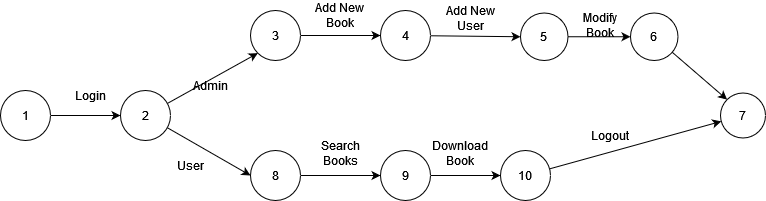
\includegraphics[width=\paperwidth]{C:/Users/Mina Sameh/Downloads/Tex/Pert.png}
}
\subsection{Gant}
\noindent\makebox[\textwidth]{
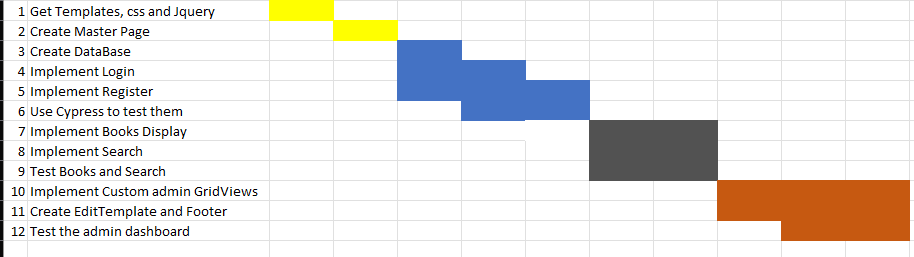
\includegraphics[width=\paperwidth]{C:/Users/Mina Sameh/Downloads/Tex/Gant.png}
}
\subsection{Class}
\noindent\makebox[\textwidth]{
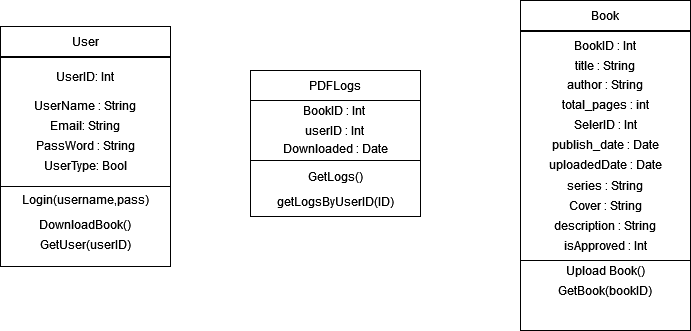
\includegraphics[width=\paperwidth]{C:/Users/Mina Sameh/Downloads/Tex/Project_Class_Diagram.png}
}
\subsection{Function}
\noindent\makebox[\textwidth]{

\includegraphics[width=\paperwidth]{C:/Users/Mina Sameh/Downloads/Tex/Project_Function_Diagram.png}
}
\subsection{State}
\noindent\makebox[\textwidth]{
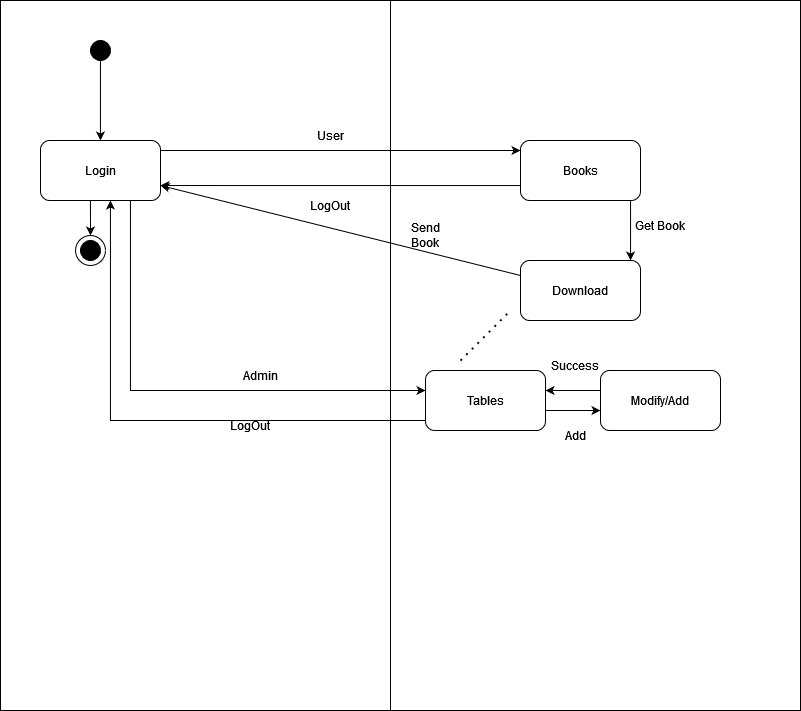
\includegraphics[width=\paperwidth]{C:/Users/Mina Sameh/Downloads/Tex/Project_State_Diagram.png}
}
\subsection{Schema}
\noindent\makebox[\textwidth]{
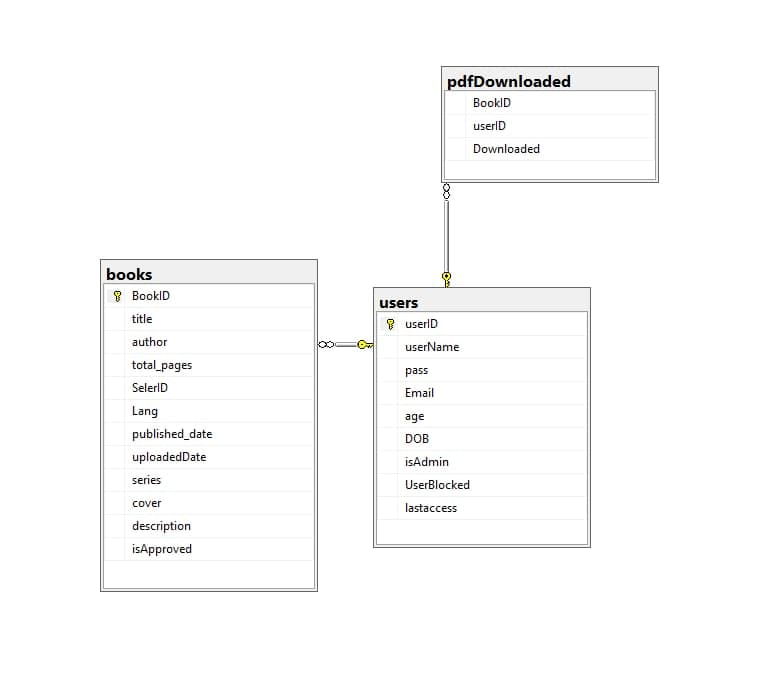
\includegraphics[width=\paperwidth]{C:/Users/Mina Sameh/Downloads/Tex/Schema.png}
}
\subsection{Sequence}
\noindent\makebox[\textwidth]{

\includegraphics[width=\paperwidth]{C:/Users/Mina Sameh/Downloads/Tex/SequenceDiagram1.png}
}
\subsection{Use Case}
\noindent\makebox[\textwidth]{
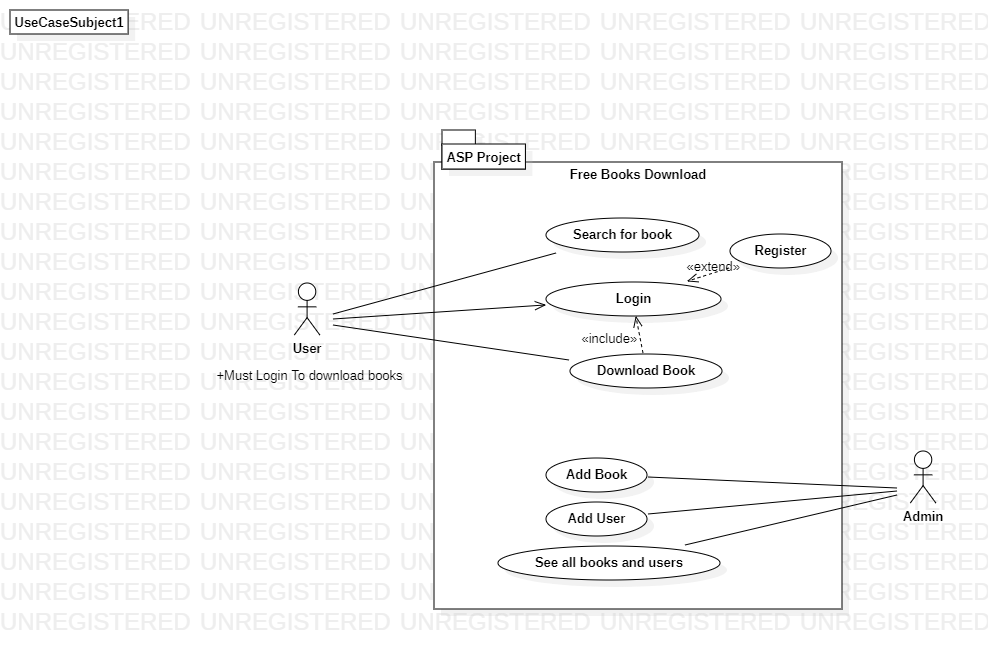
\includegraphics[width=\paperwidth]{C:/Users/Mina Sameh/Downloads/Tex/UseCaseDiagram.png}
}

\section{Future Work}
Wanted to Show the pdfs that were Downloaded by user and sort them etc but didn't have enough time sadly.\\
Wanted to make a masterPage sepreate for the admin but couldn't find  a good one.\\

\section*{End}

Special Thanks to Eng Hadeer.



\end{document}

